\documentclass{article}

% Language setting
% Replace `english' with e.g. `spanish' to change the document language
\usepackage[english]{babel}

% Set page size and margins
% Replace `letterpaper' with`a4paper' for UK/EU standard size
\usepackage[letterpaper,top=2cm,bottom=2cm,left=3cm,right=3cm,marginparwidth=1.75cm]{geometry}
\usepackage{amsmath}

% Useful packages
\usepackage{amsmath}
\usepackage{amsfonts}
\usepackage{graphicx}
\usepackage[Symbol]{upgreek}
\usepackage[colorlinks=true, allcolors=blue]{hyperref}

\title{Hamilton-Jacobi Reachability}
\author{Kai Yun}

\begin{document}
\maketitle

\section{Backward Reachability Set (BRS)}

\quad A BRS represents the set of states $x \in {\rm I\!R}^n$ from which the system can be driven into some set $\mathcal{G}_{0} \subseteq {\rm I\!R}^n$ at the \textit{end} of a time horizon of duration $|t|$, where $\mathcal{G}_{0}$ is called the ``target set". \\
\begin{itemize}
    \item Player 1 tries to steer the system away from the target with input $a(\cdot).$
    \item Player 2 tries to steer the system toward the target with input $b(\cdot).$
\end{itemize}

\begin{figure}[h]
\centering
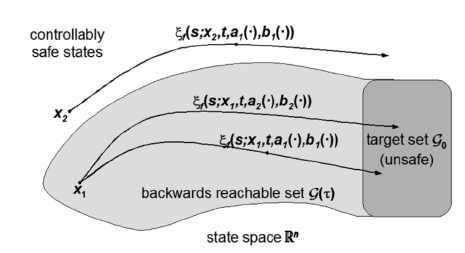
\includegraphics[width=0.6\textwidth]{BRS.PNG}
\caption{Target set and backward reachable set. Input signal $a(\cdot)$ is chose to drive the trajectory away from the target set, while input signal $b(\cdot)$ is chose to drive the trajectory toward the target.}
\end{figure}

\subsection{System Dynamics}
\begin{align}
\dot{x}(s) = f(x(s), a(s), b(s))
\end{align}

\begin{itemize}
    \item $s\in[t,0],\ a(s) \in \mathcal{A} \subset {\rm I\!R}^{n_u},\ b(s) \in \mathcal{B} \subset {\rm I\!R}^{n_d}$ where $\mathcal{A}$ and $\mathcal{B}$ are control inputs, compact and $t < 0$.
    \item $a(s)$ and $b(s)$ denote the input for Player 1 and Player 2.
    \item $x \in  {\rm I\!R}^n$ is the system state and evolves according to the ODE, (1).
    \item System dynamics (i.e., flow field), $f: {\rm I\!R}^n \times \mathcal{A} \times \mathcal{B}$, is assumed to be uniformly continuous, bounded, and Lipschitz continuous in $x$ uniformly in $a(\cdot)$ and $b(\cdot)$.
\end{itemize}

\newpage

\subsection{Trajectories of (1)}
\quad Due to the conditions of the system dynamics stated above, given $a(\cdot) \in \mathbb{A}$ and  $b(\cdot) \in \mathbb{B}$, there exists a unique trajectory solving (1). Here, $\mathbb{A}$ and $\mathbb{B}$ are sets of ``measurable functions" that maps $s$ to control inputs $\mathcal{A}$ and $\mathcal{B}$. \\
The solutions, or trajectories of (1) starting from state $x$ at time $t$ under control $a(\cdot)$ and $b(\cdot)$ is: $\upzeta(s;x,t,a(\cdot),b(\cdot)) \ : \ [t,0] \rightarrow {\rm I\!R}^n$. \\
$\upzeta$ satisfies (1) with an initial condition almost everywhere:

\begin{equation}
\begin{aligned}
\frac{d}{ds}\upzeta(s;x,t,a(\cdot),b(\cdot)) & = f(\upzeta(s;x,t,a(\cdot),b(\cdot)),a(s),b(s))\\
\upzeta(t;x,t,a(\cdot),b(\cdot)) & = x
\end{aligned}
\end{equation}

The second line in equation (2), literally just means ``the trajectory of the system starting from state $x$ at time $t$, and ending at time $t$ is $x$."

\subsection{Backward Reachability Set $\mathcal{G}$}
\quad To reiterate, the control input $a(\cdot)$ aims to drive the system \textbf{away} from the target, while $b(\cdot)$ aims to drive the system \textbf{toward} the target. Accordingly, the BRS we'd like to compute is the following:

\begin{equation}
\begin{aligned}
\mathcal{G}(t) = & \{x: \exists \upgamma \in \Upgamma(t), \forall a(\cdot) \in \mathbb{A},\\
& \upzeta(0;x,t,a(\cdot), \upgamma[a](\cdot)) \in \mathcal{G}_0\}
\end{aligned}
\end{equation}
\\
where $\Upgamma(\cdot)$ denotes the feasible set of strategies for Player 2.
\\
\quad Thus, BRS is a set of system states $x$ that eventually leads the trajectory $\upzeta$ starting from $x$ at time $t$ to the unsafe ``target set" $\mathcal{G}_0$, according to control inputs $a(\cdot)$ and $b(\cdot)$. \textbf{However}, this particular BRS - the one we want to compute - is the set that \textbf{inevitably} leads to the unsafe target set no matter the control input $a(\cdot)$ due to the well-calculated(?) control input $\upgamma$. The computation of the BRS in (3) requires solving a differential game between Player 1 and Player 2.

\subsection{Non-anticipative Strategies $\Upgamma(\cdot)$ of Player 2}
\quad Player 2 only uses non-anticipative strategies $\Upgamma(\cdot)$ in reachability problems.

\begin{equation}
    \begin{aligned}
    \upgamma \in \Upgamma(t) & := \{\mathcal{N} : \mathbb{A}(t) \rightarrow \mathbb{B}(t) : a(r) = \hat{a}(r) \ \text{a.e.} \ r \in [t,s] \\
    & \Rightarrow \mathcal{N}[a](r) = \mathcal{N}[\hat{a}](r) \ \text{a.e.} \ r \in [t,s]\}
    \end{aligned}
\end{equation}

Player 2 cannot respond differently to two Player 1 controls until they become different. Yet, Player 2 has the advantage of factoring in Player 1's choice of input at every instant $t$ and adapting its own accordingly (i.e. Player 2 cannot anticipate, but can adapt!). Thus, Player 2 has an \textit{instantaneous informational advantage}, which allows us to establish safety guarantees under the worst-case scenarios (???). \\
\\

\subsection{Game of Kind vs Degree}
\begin{itemize}
    \item Game of Kind: Game in which the outcome is determined by \textit{whether or not} the state of the system reaches a given configuration under specified constraints at any time within the duration of the game.
    \item Game of Degree: Game in which the outcome is determined by \textit{the degree} the state of the system reaches under specified constraints at any time within the duration of the game (???).
\end{itemize} 

\quad Now, the differential game that must be solved in order to compute the BRS in (3) is a ``game of kind" rather than a ``game of degree".
\textit{\textbf{Level set method}} can transform these games of kind into games of degree in an analytically sound and computationally tractable way.

\section{Two-Person Zero-sum Differential Games}

\subsection{Cost Function}
\quad Often, the goal is to optimize a cost function of the final state and some running cost or reward accumulated over system trajectories.\\
\quad Let $J_t(x, a(\cdot), b(\cdot))$ denote the cost accumulated during horizon $[t,0]$ when Player 1 and Player 2 play control $a(\cdot)$ and $b(\cdot)$, respectively.

\begin{align}
    J_t(x, a(\cdot), b(\cdot)) = \int_{t}^{0} c(x(s), a(s), b(s), s) \, ds + q(x(0))
\end{align}

In the zero-sum setting, Player 1 will attempt to maximize this outcome, while the Player 2 will aim to minimize it, subject to the system dynamics in (1).

\subsection{Lower Value of the Game}
\quad Under the non-anticipative strategy assumption, the \textit{lower value} of the game can be defined as the following:

\begin{align}
    G(t,x) = \inf_{\upgamma \in \Upgamma(t)} \sup_{a(\cdot) \in \mathbb{A}} J_t(x, a(\cdot), \upgamma[a](\cdot))
\end{align}
\\
where $\Upgamma(\cdot)$ is defined in (4). (Note that, in general, for the scenarios that we're interested in, the lower value itself will suffice without the upper value.)

\subsection{Hamilton-Jacobi Isaacs (HJI)}
Using dynamic programming, it can be shown that the value function $G(t,x)$ in (6) is the viscosity solution of the following HJI PDE:

\begin{equation}
    \begin{aligned}
    & D_tG(t,x) + H(t,x,\nabla G(t,x)) = 0 \\
    & G(0,x) = q(x)
    \end{aligned}
\end{equation}
\\
where $H(t,x, \nabla G(t,x))$ is called the \textit{\textbf{Hamiltonian}} and is defined as:
\begin{align}
    H(t,x,\lambda) = \max_{a \in \mathcal{A}} \min_{b \in \mathcal{B}} c(x,a,b,t) + \lambda \cdot f(x,a,b)
\end{align}
\\
where $\lambda$ in (8) denotes $\nabla G(t,x)$ and is called the \textit{costate}.

\subsection{Optimal Control for Player 1}
Given the value function, the optimal control for Player 1 is:

\begin{align}
    a^{*}(t,x) = \text{arg}\max_{a \in \mathcal{A}} \min_{b \in \mathcal{B}} c(x,a,b,t) + \lambda \cdot f(x,a,b).
\end{align}
\\
The optimal control for Player 2 can be similarly obtained.

\newpage

\section{The Level Set Approach}
\quad The differential games of degree can be solved using an HJ PDE. However, the computation of the BRS is a differential game of kind where the outcome is Boolean: the system either reaches the target set or not. We can ``encode" this Boolean outcome through a quantitative value function:
for example, if we consider $J_t(\cdot)$ as the distance between the system state and the target region at the terminal state of the system, it is easy to determine whether the system reached the target by comparing this distance to some threshold value (simply 0 in this case). This allows us to find the solution to a game of kind by posing an auxiliary game of degree whose solution encodes that of the original problem: this is, in essence, the level set approach.

\subsection{Lipschitz Function: Cost Function}
\quad One can always find a Lipschitz Function $g(x)$ such that $\mathcal{G}_0$ (target set) is equal to the zero sublevel set of $g$, that is, $x \in \mathcal{G}_0 \iff g(x) \leq 0$, i.e. state $x$ is in the target set if and only if the target set is equal to the zero sublevel set of $g$.\\
\quad The Lipschitz function $g$ can always be found, since one can always choose the signed distance to the respective sets.\\
\quad If the cost function is defined as
\begin{align}
    J_t(x,a(\cdot), b(\cdot)) = g(x(0)),
\end{align}
\\
then the system reaches the target set under controls $a$ and $b$ if and only if $J_t(x,a(\cdot),b(\cdot) \leq 0$. 

\subsection{Optimization for Each Player}
\begin{itemize}
    \item Player 1 wants to drive the system \textbf{away} from the target, and thus wants to maximize the cost (10).
    \item Player 2 wants to drive the system \textbf{toward} the target, and thus wants to minimize the cost (10).
\end{itemize}

Now, we can compute the value function $G(t,x)$ for this differential game as done in equations (6) ~ (9). The BRS can be obtained as
\begin{align}
    \mathcal{G}(t) = \{ x: G(t,x) \leq 0 \}
\end{align}\\
where $G(t,x)$ satisfies the following HJI PDE:
\begin{equation}
    \begin{aligned}
    & D_tG(t,x) + H(t,x,\lambda) = 0
    & G(0,x) = g(x).
    \end{aligned}
\end{equation}
\\
The Hamiltonian is given by:
\begin{align}
    H(t,x,\lambda) = \max_{a \in \mathcal{A}} \min_{b \in \mathcal{B}} \lambda \cdot f(x,a,b).
\end{align}

\subsection{Interpretation of $\mathcal{G}(t)$}
\begin{itemize}
    \item \textbf{$x(t) \in \mathcal{G}(t)$}: Player 2 has a control sequence that will drive the system to the target at time 0, irrespective of the control of Player 1.
    \item \textbf{$x(t) \in \partial \mathcal{G}(t)$}: ($\partial \mathcal{G}(t)$ denotes the boundary of $\mathcal{G}(t)$) Player 1 will \textit{barely} miss the target at time 0 if it applies the optimal control
        \begin{align}
            a^*(t,x) = \text{arg} \max_{a \in \mathbb{A}} \min_{b \in \mathbb{B}} \lambda \cdot f(x,a,b).
        \end{align}
    \item \textbf{$x(t) \in \mathcal{G}(t)^C$}: Player 1 has a control sequence (given by (14)) that will keep the system out of the target set, irrespective of the control applied by Player 2.
\end{itemize}

\newpage

To summarize, $\mathcal{G}(t)$ represents the \textit{effective} unsafe set, i.e. the set of states from which the disturbance can drive the system to the \textit{actual} unsafe set despite the best control efforts. Here, $\mathcal{G}_0$ represents the unsafe states of the system and Player 2 represents the disturbances in the system.
\\
\\
$\Longrightarrow$ Reachability analysis gives us the safe set (in this case $\mathcal{G}(t)^C$ as well as a controller (in this case $a^*(t,x)$) taht will keep the system in the safe set, give nthat the system starts in the safe set.

\section{Different Reachability Analysis Methods}
Reachability analysis is not limited to BRSs. One can compute various other kinds of sets, depending on the verificiation problem at hand.

\subsection{Forward vs Backward Reachable Set}
\quad \textbf{Forward Reachable Set (FRS)}: the set of all states that a system can reach from a given initial set of states after a time duration of $|t|$.
\begin{equation}
    \begin{aligned}
    \mathcal{W}(t) = & \{ y : \exists \upgamma \in \Upgamma(t), \forall a(\cdot) \in \mathbb{A}, \\
    & \upzeta (t;x,0,a(\cdot),\upgamma[a](\cdot)) = y, \ x\in \mathcal{G}_0\}, t > 0.
    \end{aligned}
\end{equation}

``For all control input of Player 1, there exists a control input of Player 2, based on its non-anticipative strategy, that directs the trajectory to $y$ at time $t$, given that the system started in one of the states $x \in \mathcal{G}_0$ at time 0."

\begin{itemize}
    \item $\mathcal{G}_0$ represents the set of initial states of system.
    \item $\mathcal{W}(t)$ is the set of all states that system can reach in a duration of $t$.
    \item Player 1 applies the control $a(\cdot)$ to keep the system in $\mathcal{G}_0$.
    \item Player 2 applies the control to drive the system out of $\mathcal{G}_0$.
\end{itemize}

The FRS can be computed in a similar fashion as the BRS. However, an \textit{initial} value HJ PDE needs to be solved instead of a final value PDE, which can always be converted into an equivalent final value PDE by change of variables.

\subsection{Reachable Sets vs. Tubes}
\begin{itemize}
    \item Reachable Set: the set of states from which the system can reach a target at \textit{exactly} time 0.
    \item Reachable Tube: the set of states from which the system can reach a target \textit{within} a duration of $|t|$. For example, for safety analysis, we are interested in verifying if a disturbance can drive the system to the unsafe states \textit{ever} within a horizon, and not just at the end of the horizon.
\end{itemize}

The formal definition of backward reachable tube (BRT) (forward reachable tube (FRT) can be similarly defined):
\begin{align}
    \mathcal{G}(t) = & \{ x : \exists \upgamma \in \Upgamma(t), \forall a(\cdot) \in \mathbb{A}, \\
    & \exists s \in [t,0], \upzeta(s;x,t,a(\cdot), \upgamma[a](\cdot)) \in \mathcal{G}_0\}.
\end{align}
The BRT can be computed by solving a final value PDE similar to that in (12).

\subsection{Roles of the Control and Disturbance}
\begin{itemize}
    \item Whenever the existence of a control (``$\exists a$") is sought, the optimization is a \textbf{minimum} over the set of controls in the corresponding Hamiltonian.
    \item Whenever a set/tube characterizes the behavior of the system for all controls (``$\forall a$"), the optimization is a \textbf{maximum} over the set of controls in the corresponding Hamiltonian.
\end{itemize}

When the target set represents the set of the desired states that we want the system to reach and Player 2's control represents the disturbance, then we are interested in verifying if there exists a control of Player 1 such that the system reaches its target despite the worst-case disturbance. In this case, we should use maximum for Player 2's control and minimum for Player 1's control in the corresponding Hamiltonian.

\subsection{Presence of State Constraints}
The reachability to and from a target set subject to some state constraints can be handled efficiently for even time-dependent constraints within the reachability framework. In general, any combination of the above four variants can be solved using the HJ reachability formulation.

\newpage
\section{Notes from Video}

\subsection{Hamilton-Jacobi-Bellman Equation (Dynamic Programming)} 
\begin{equation}
    \begin{aligned}
        & V(x,t) = \min_{u(\cdot)}\left[ \int_{t}^{t + \delta} c(\upzeta (s;x), u(s)) \, ds + V(\upzeta(t + \delta; x), t + \delta) \right] \\
        & V(x,T) = l(x)
    \end{aligned}
\end{equation}
This equation, the Hamilton-Jacobi-Bellman (HJB) Equation, allows us to calculate the value function starting "backwards", like a recursive function. We first calculate the running cost, $c$, up to our current timestep $t+\delta$ from the starting timestep $t$. Then, we recursively add the value function starting from the current timestep and ending at the final trajectory $\upzeta(t + \delta; x)$. The value function at the terminal timestep $T$ is simply $V(x,T) = l(x)$ where $l(x)$ is the terminal cost of the optimal control.
\\
\\
An equivalent form of HJB PDE in differential form is as follows:
\begin{equation}
    \begin{aligned}
    & \frac{dV}{dt} + \min_{u} \{ \nabla V(x,t) \cdot f(x,u) + c(x,u) \} = 0 \\
    & V(x,T) = l(x)
    \end{aligned}
\end{equation}
At least for this tutorial, \textbf{Optimal Control == Solving a HJB PDE}.

\subsection{Zero-sum Differential Games}
Now, there is one more player in this dynamics, namely \textit{disturbance}. The cost function follows as:

\begin{equation}
    \begin{aligned}
        & J_0(x,u(\cdot), d(\cdot)) =  \int_{0}^{T} c(\upzeta (s;x), u(s), d(s)) \, ds + l(\upzeta(T; x)) \\
        & \dot{x} = f(x,u,d)
    \end{aligned}
\end{equation}
where $u$ is the \textbf{control} for Player I and $d$ is the \textbf{disturbance} for Player II. Player I strives to minimize the cost and Player II tries to maximize the cost. 
\\
\\
\quad Note that Player II uses non-anticipative strategies, as explained in section 1.4. What that means is that "future action of Player I does NOT affect the current actions of Player II." In some sense, this means that the game is evolving continuously, i.e. the two players are playing continuously, not in discrete time. 
\\
The value function for this game is:


\newpage

\section{Background Knowledge}

\subsection{Partial Differential Equation (PDE)}

\subsection{Differential Game}
The extension of sequential game theory to the \textit{continuous-time} case is called \textbf{\textit{differential game theory}} (or \textit{dynamic game theory}), a subject introduced by Rufus Isaacs. The following variants are possible:
\begin{enumerate}
    \item There may be any number of players.
    \item The game may be zero-sum or nonzero-sum.
    \item The state may or may not be known. If the state is unknown, then interesting I-spaces arise.
    \item Nature can interfere with the game.
    \item Different equilibrium concepts, such as saddle points and Nash equilibria, can be defined. 
\end{enumerate}

Two players, $P_1 \text{and} P_2$, can be engaged in a \textit{differential game} in which each has a continuous set of actions. A state transition equation can be defined as
\begin{align}
    \dot{x} = f(x,u,v)
\end{align}
in which $x$ is the state, $u \in U$, and $v \in V$ where $U$ and $V$ denote the action spaces of $P_1$ and $P_2$, respectively. Note that \textit{linear differential games} are an important family of games because many techniques from optimal control theory can be extended to solve them.




\end{document}